\chapter{OpenVAS Scan}

\label{cha:openvas_scan}


\section{OpenVAS Scan}
In this section it will be explained how to start a scan (that could be just for an host, or a group of hosts). We will create a target, which means declaring which host (or group of hosts) to be scanned, which port range and protocol. 

\begin{figure}[H]
    \centering
    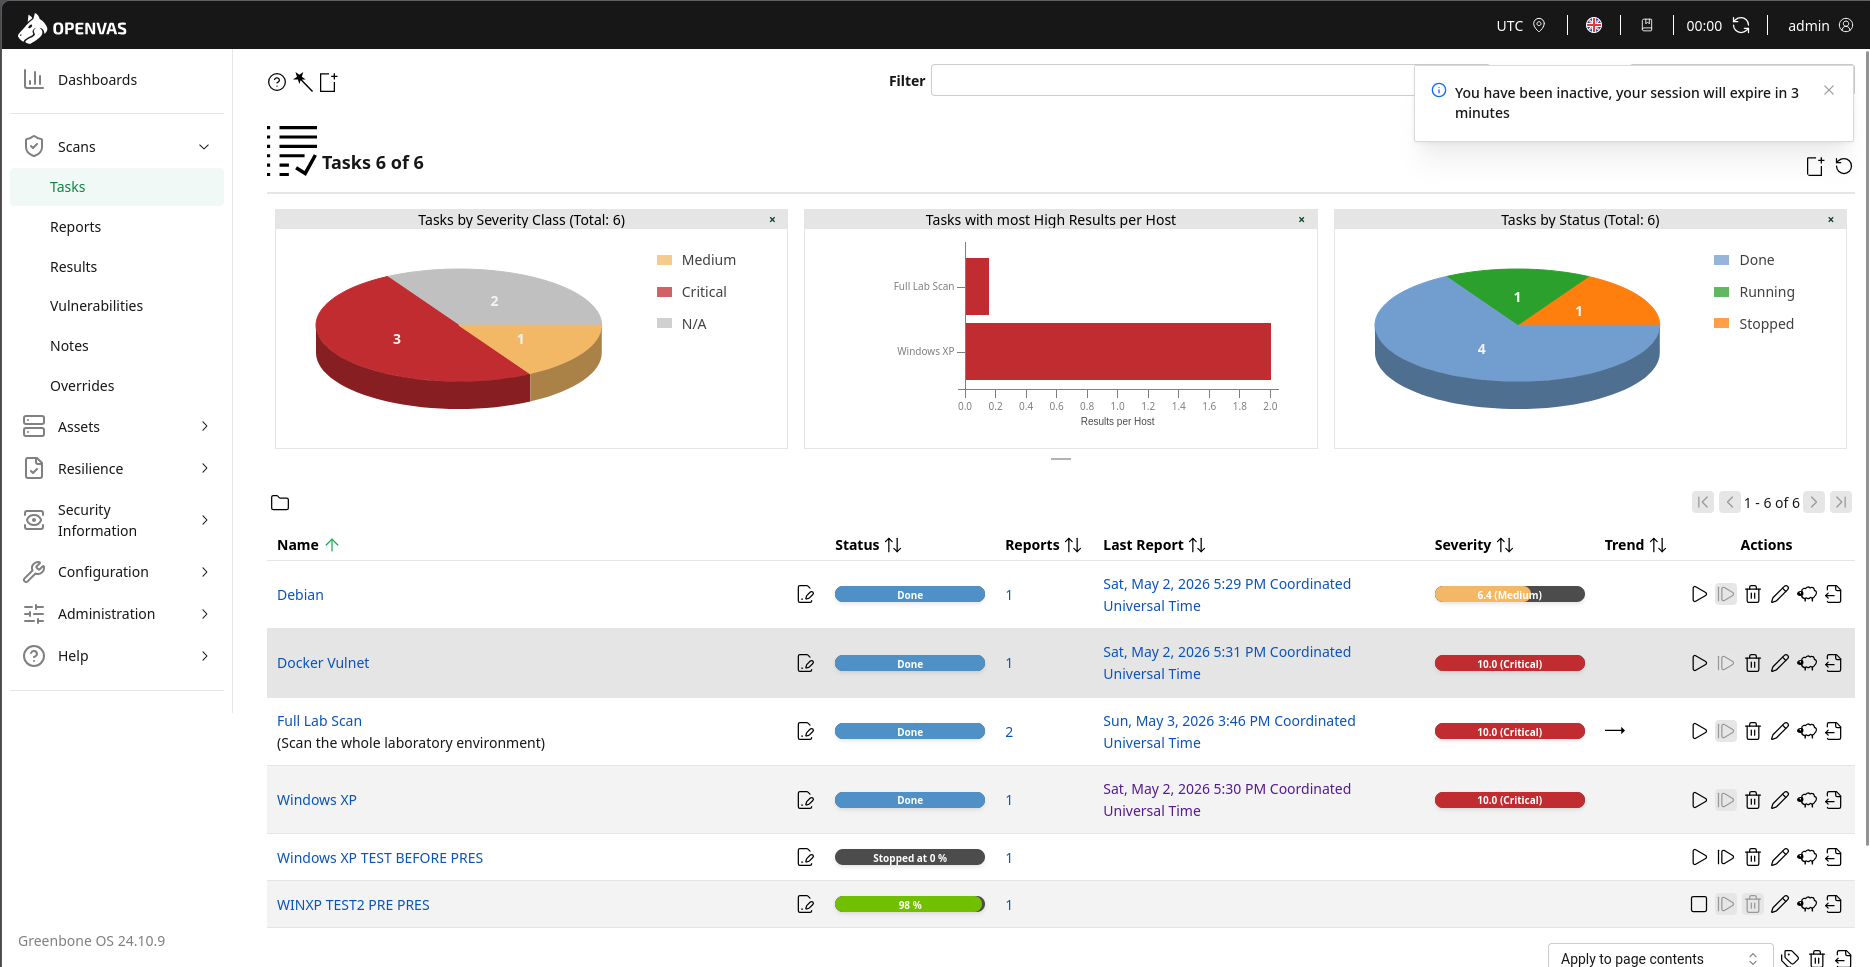
\includegraphics[width=0.9\textwidth]{../presentation/images/openvas_scan_interface1.png}
    \caption{Scan windows}
\end{figure}

This is the scan windows, where you will create the tasks which are configurations for the targets and ports that are going to be scanned, how many NVTs (Network Vulnerability Test) are going to be used for the scan, how many concurrent hosts are being scanned at a given moment etc. We will get to all of the configuration in time.

\subsection{Configuration $\rightarrow$ Ports}

\begin{figure}[H]
    \centering
    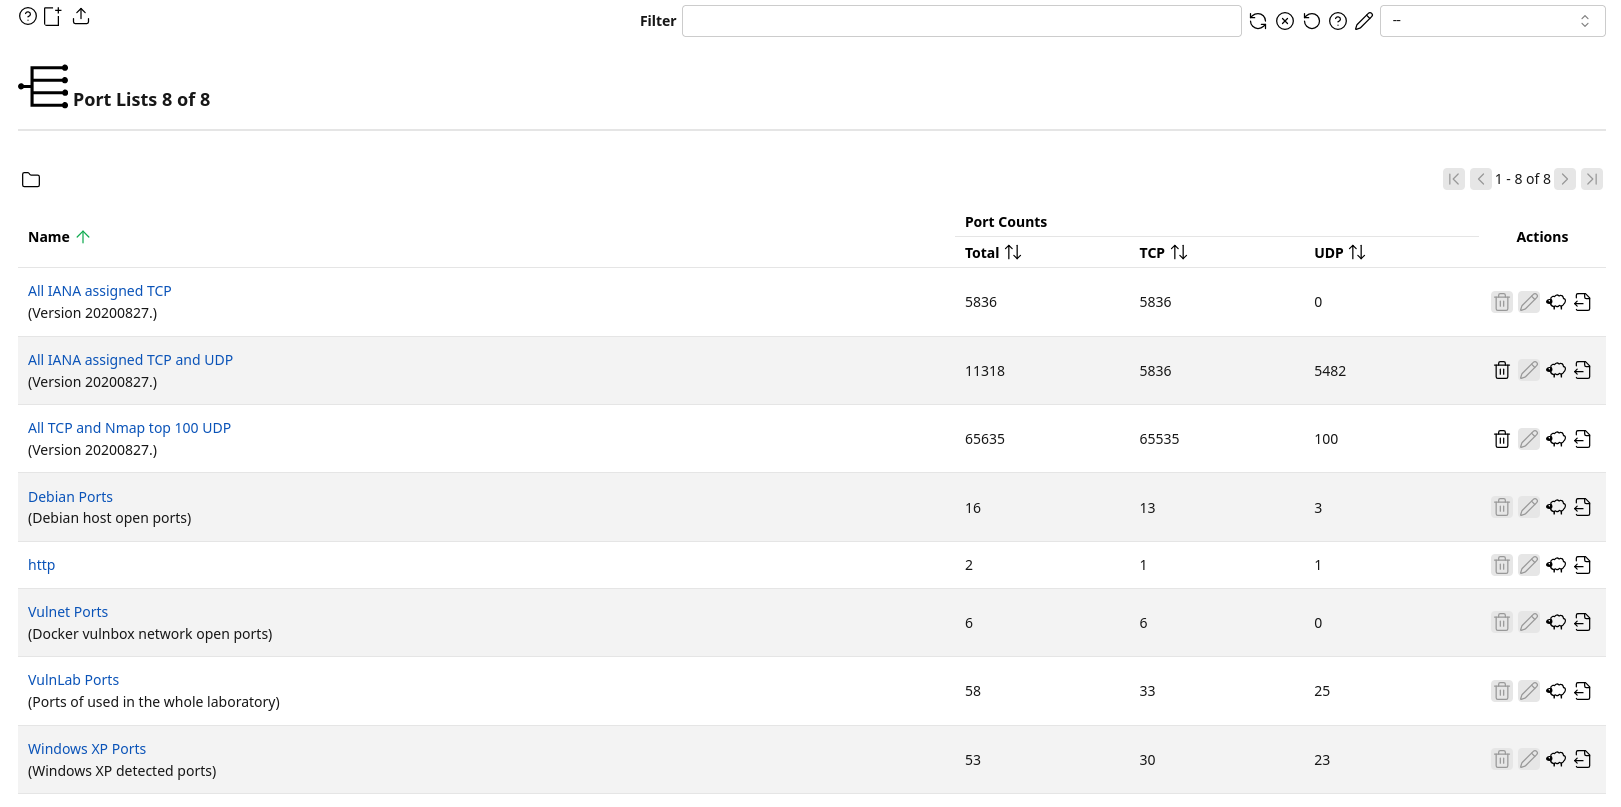
\includegraphics[width=0.9\textwidth]{../presentation/images/openvas_ports_interface1.png}
    \caption{Port creation interface}
\end{figure}




This is the ports creation interface, you can create custom ports ranges looking for services that use TCP/UDP. For the most part OpenVAS works by giving us templates, in this case are for a complete scans of all IANA (Internet Assigned Numbers Authority) ports, which means it will scan for all $65536$ ports only TCP, UDP, both etc. It really just depends on which preset is chosen. 

OpenVAS encodes ports in a format like T:$1-1023$, $4500$,U:$2-100$, $3246$ which means that it will scan for TCP ports between $1$ and $1023$ and 4500 alone, and for UDP ports from $2$ to $100$ and $3246$ alone. In this way you can define ports range and choose to do only TCP or UDP scans.

Under the hood OpenVAS uses Nmap to scan the ports, and just like it to scan UDP ports it will take considerably longer than TCP. This is because when a TCP request is made, the server either accept the connection or it rejects it, while for UDP being a connection-less protocol will wait until timeout. So beware about this aspect if you don't want the scan to take hours. 

For our experiments we will create two presets: one for ftp service (port $21$) and one for an http server (port $80$). Go on the add port icon on the top of the interface (the little square with a plus), and you should get this popup.

% \begin{figure}[H]
%     \centering
%     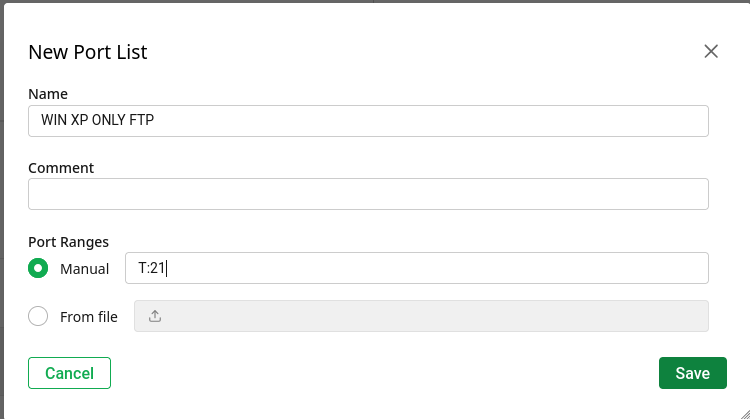
\includegraphics[width=0.8\textwidth]{images/openvas_xpftp.png}
%     \caption{Port configuration limited to \texttt{TCP 21} (FTP).}
% \end{figure}

% To configure the ports click on the add button on the top of the page.


% \begin{figure}[H]
%     \centering
%     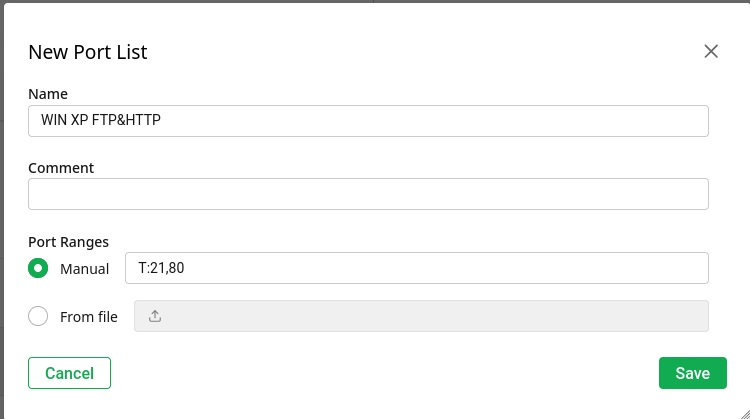
\includegraphics[width=0.8\textwidth]{images/openvas_xpftphttp.png}
%     \caption{Port configuration limited to \texttt{TCP 21 and 80} (FTP).}
% \end{figure}



\begin{figure}[H]
    \centering
    \begin{subfigure}{0.48\textwidth}
        \centering
        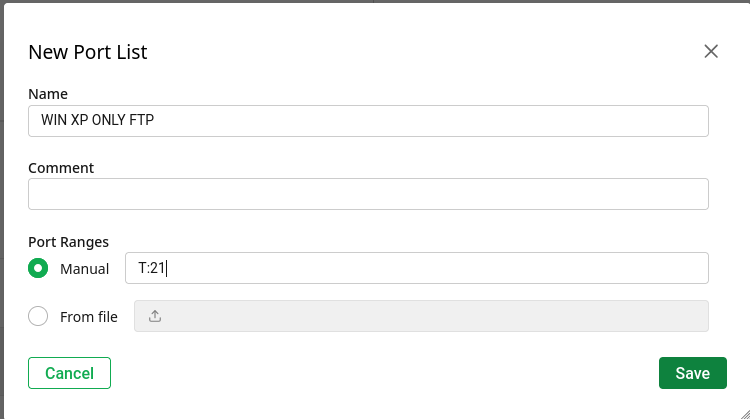
\includegraphics[width=\textwidth]{images/openvas_xpftp.png}
        \caption{Port configuration limited to \texttt{TCP 21} (FTP).} 
        \label{fig:porttarget1}
    \end{subfigure}
    \hfill 
    \begin{subfigure}{0.48\textwidth}
        \centering
        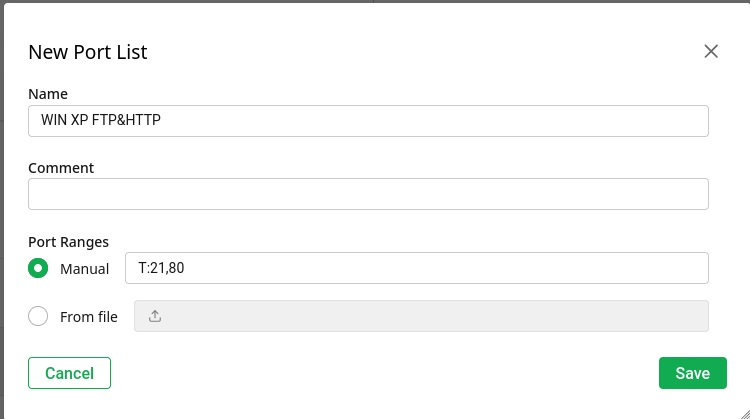
\includegraphics[width=\textwidth]{images/openvas_xpftphttp.png}
        \caption{Port configuration limited to \texttt{TCP 21 and 80} (FTP).}
        \label{fig:porttarget2}
    \end{subfigure}
    \caption{Ports configuration}
    \label{fig:port_config}
\end{figure}



Those configurations are going to be used later to scan a Windows XP target with FTP and HTTP servers.

\subsubsection{Credentials for target access}
\begin{figure}[H]
    \centering
    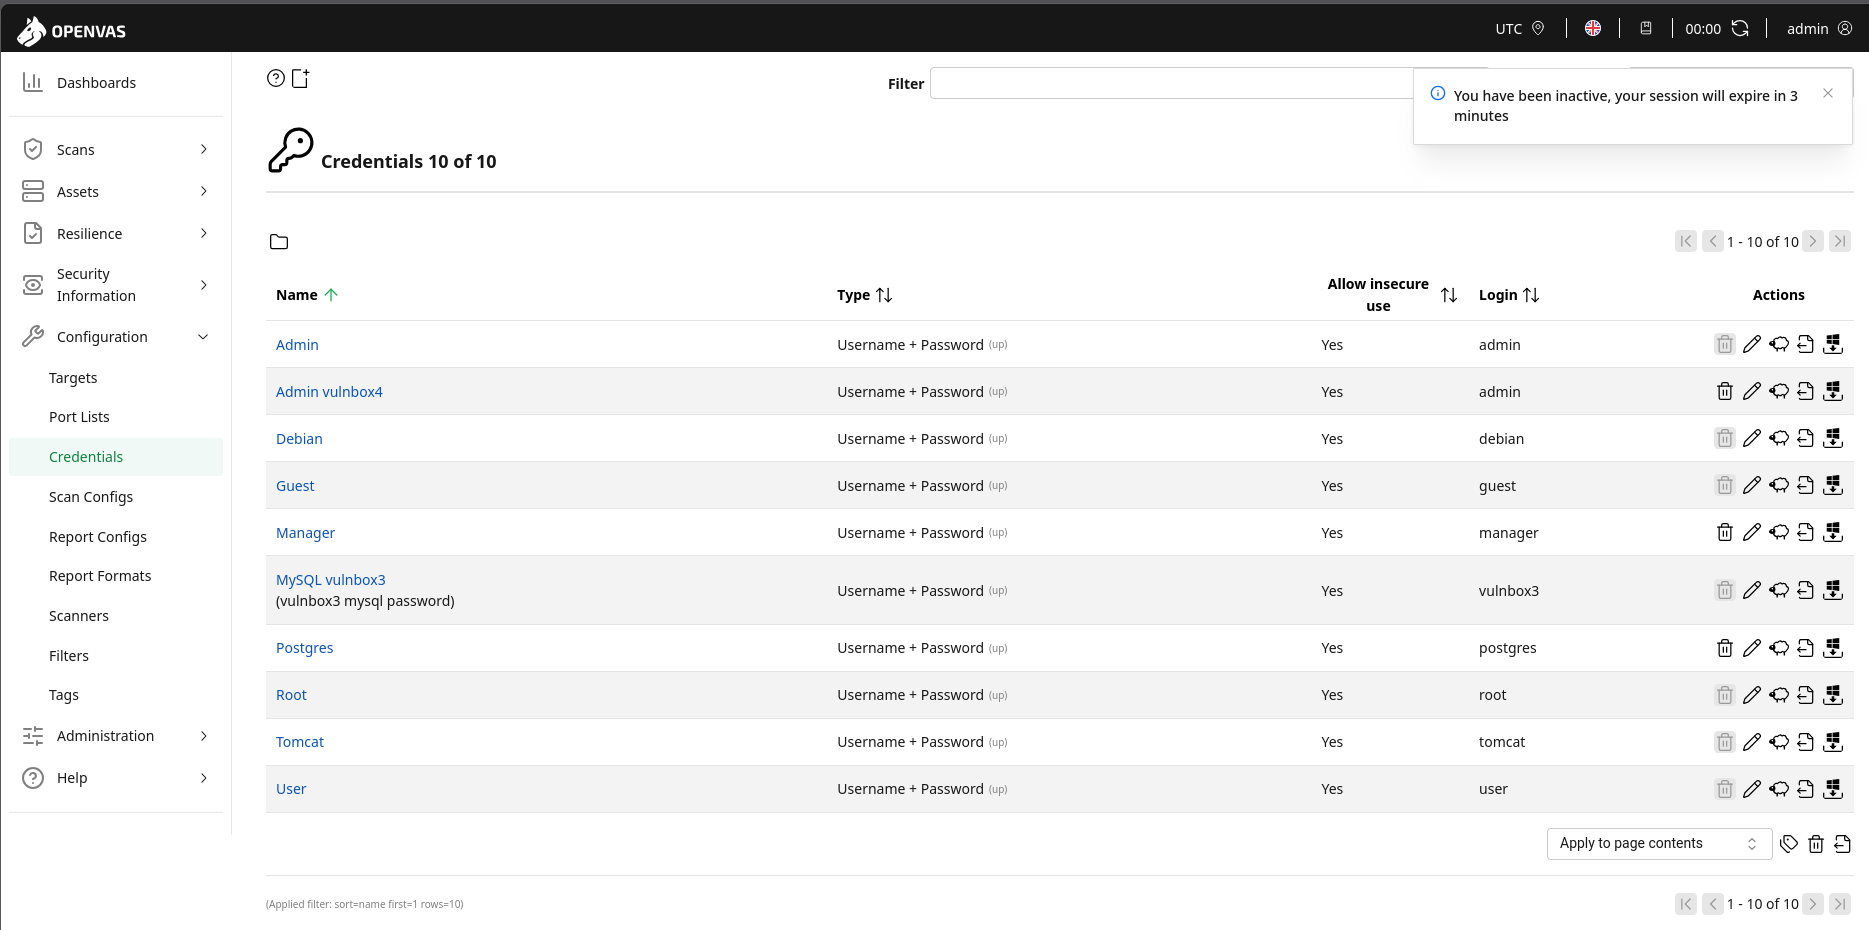
\includegraphics[width=0.8\textwidth]{images/openvas_credentials.png}
    \caption{Credentials window}
\end{figure}

Credentials are used for deeper scans, you give the credentials to OpenVAS and it will try to login to the machine, scanning the host from within, looking at configuration files, installed packages etc. This is done to improve scan performance since it flags problems that are not visible from the outside, but may lead to exploitable vulnerabilities. This function can also be used to check for default credentials if they are in use or no.

\begin{figure}[H]
    \centering
    \begin{subfigure}{0.48\textwidth}
        \centering
        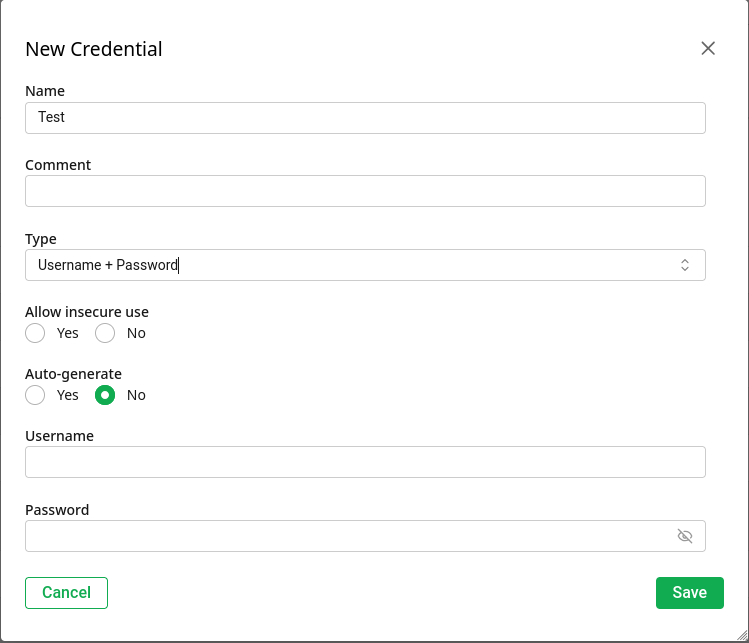
\includegraphics[width=\textwidth]{images/openvas_credentialssetup1.png}
        \caption{FTP Target Step 1} 
        \label{fig:credentialstarget1}
    \end{subfigure}
    \hfill 
    \begin{subfigure}{0.48\textwidth}
        \centering
        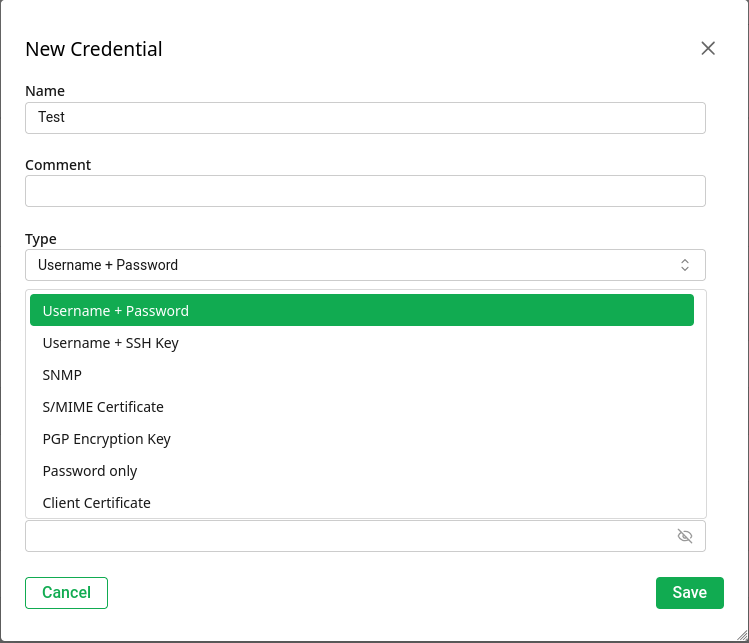
\includegraphics[width=\textwidth]{images/openvas_credentialssetup2.png}
        \caption{FTP Target Step 2}
        \label{fig:credentialstarget2}
    \end{subfigure}
    \caption{Configuration for the FTP only target}
    \label{fig:credentials_config}
\end{figure}

As you can see many possibilities are available, setting both username and password, ssh access, certificates etc. But for our example this feature will not be used.

\subsection{Target configuration}

\begin{figure}[H]
    \centering
    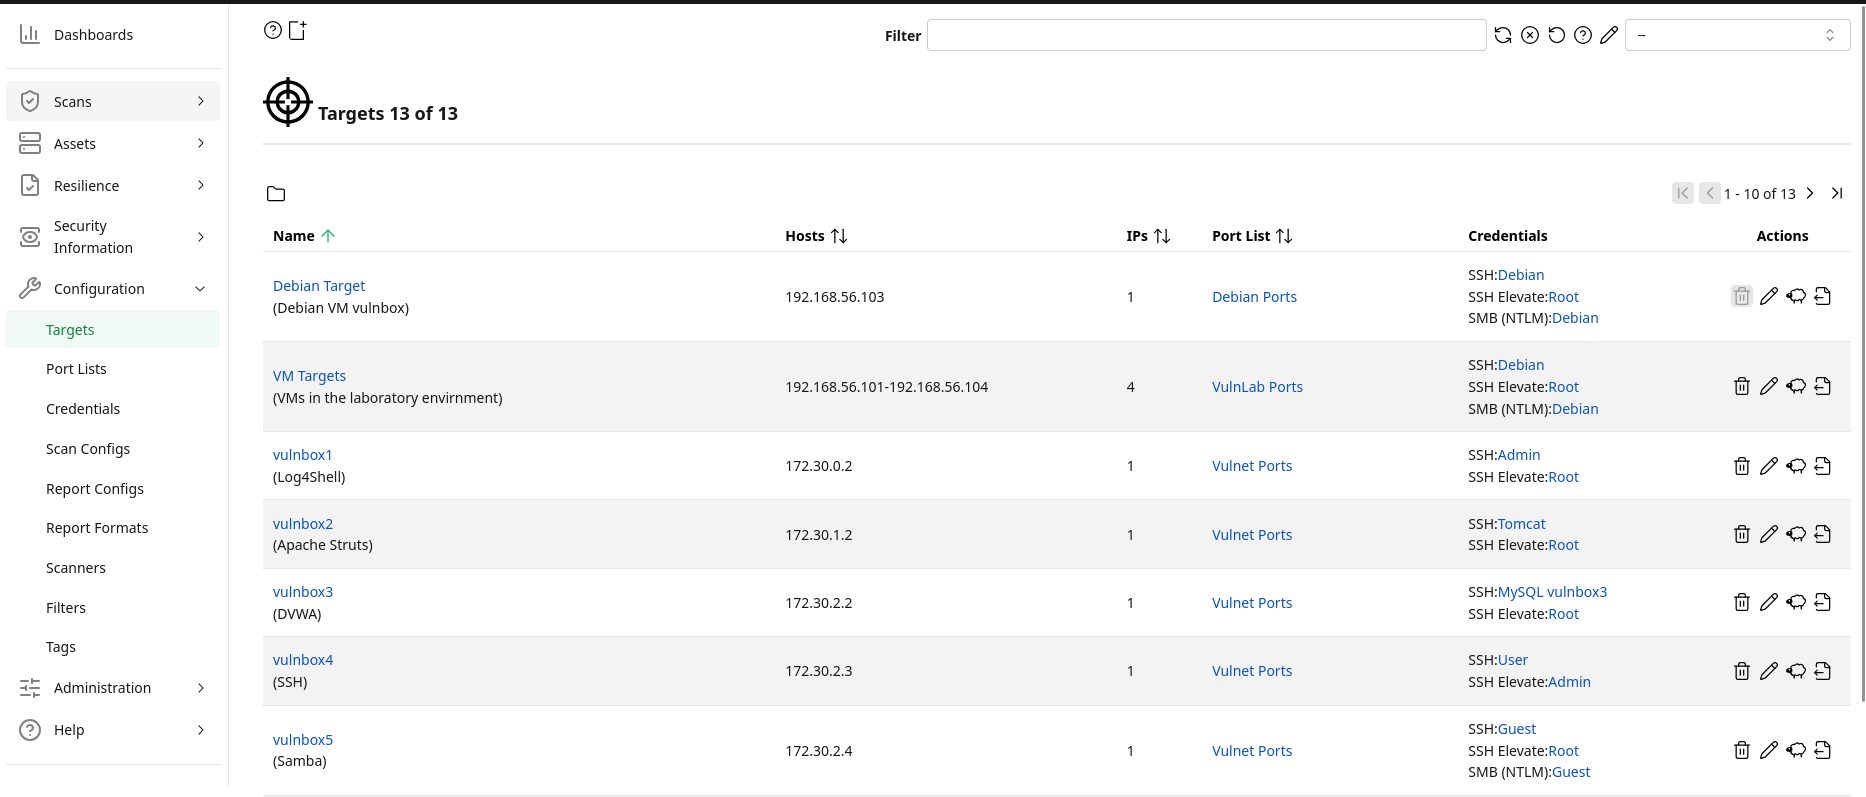
\includegraphics[width=0.9\textwidth]{../presentation/images/openvas_conftargets.png}
    \caption{Target configuration interface}

\end{figure}

This is the target creation interface, which is used to create all targets that are going to be scanned expressed in single IP or a range of IPs (e.g. 192.168.56.101-192.168.56.105). 

Before scanning the Windows XP server you would want to go to the terminal of the machine and type \textbf{ipconfig /all}, copy the IP (which should be along the lines of 192.168.56.10X).

\begin{figure}[H]
    \centering
    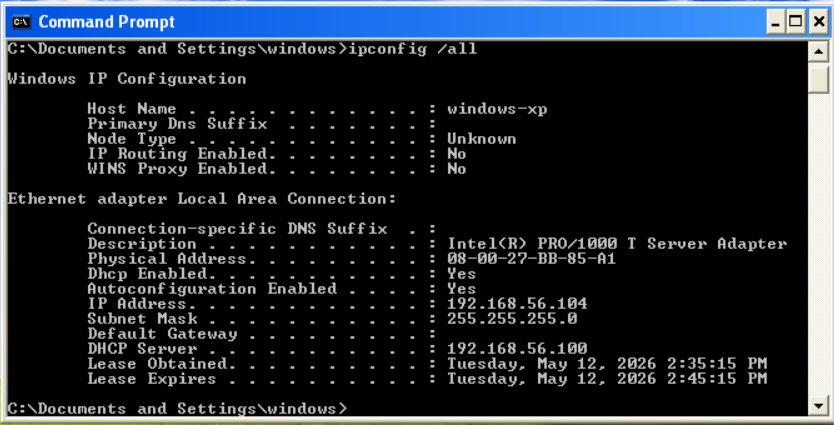
\includegraphics[width=0.8\textwidth]{images/winxp_ip.png}
    \caption{Terminal output of ipconfig command}
\end{figure}


After the IP was discovered, its time to configure the target like so:




\begin{figure}[H]
    \centering
    \begin{subfigure}{0.48\textwidth}
        \centering
        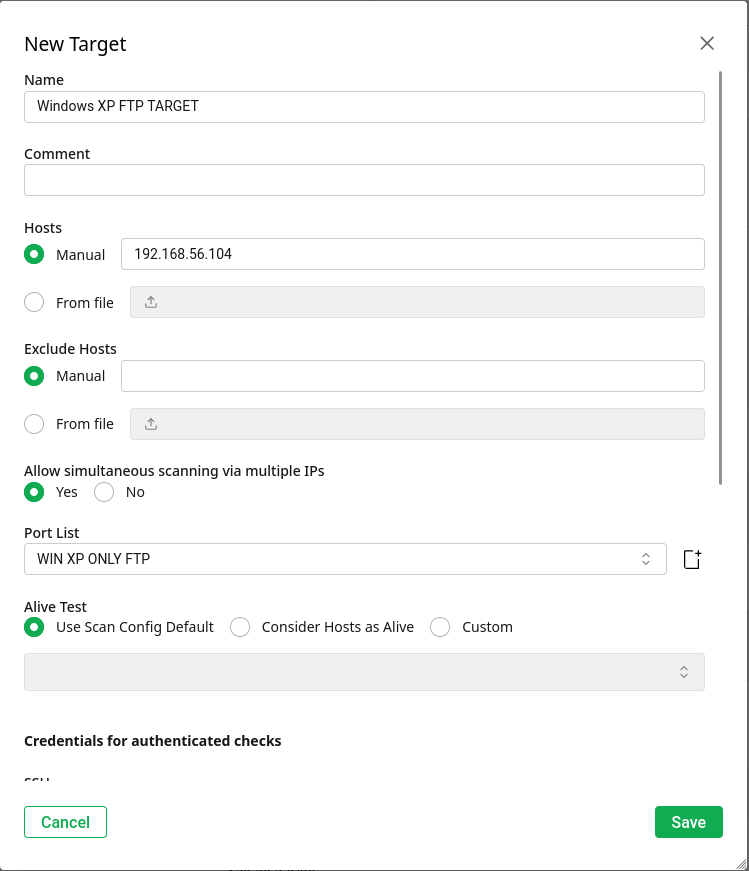
\includegraphics[width=\textwidth]{images/openvas_ftptarget1.png}
        \caption{FTP Target Step 1} 
        \label{fig:ftptarget1}
    \end{subfigure}
    \hfill 
    \begin{subfigure}{0.48\textwidth}
        \centering
        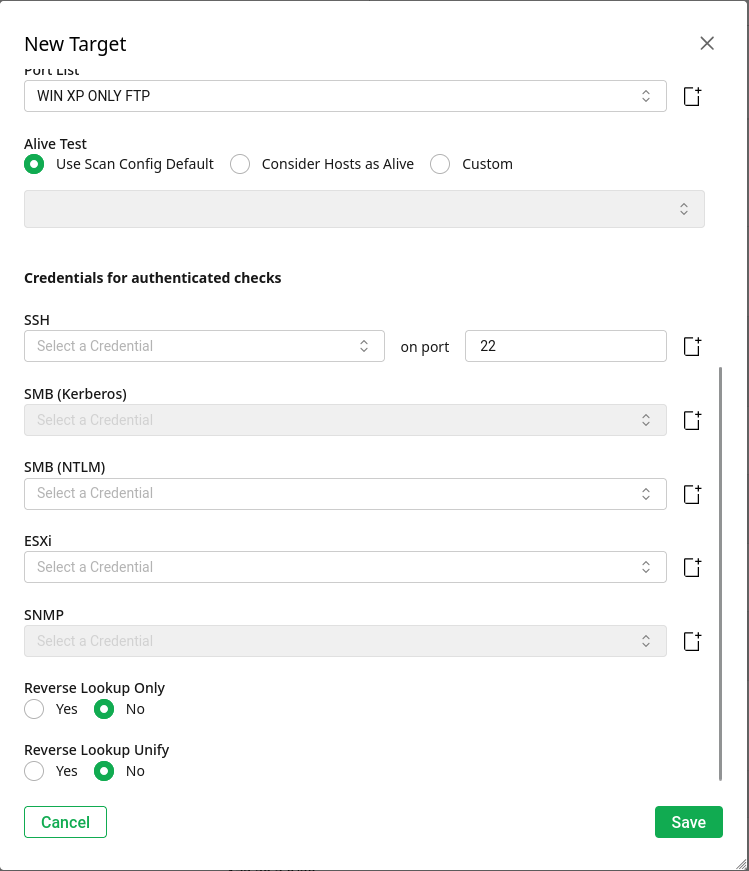
\includegraphics[width=\textwidth]{images/openvas_ftptarget2.png}
        \caption{FTP Target Step 2}
        \label{fig:ftptarget2}
    \end{subfigure}
    \caption{Configuration for the FTP only target}
    \label{fig:full_target_config}
\end{figure}

In this popup you will set target name, the IP (or range of IPs), the excluded hosts in case you have a range of IPs and some host are not to be scanned, the port list preset made before and the credentials presets that are set in the credentials window (not used in this example).


Now configure the targets also for the FTP and HTTP target like so:

\begin{figure}[H]
    \centering
    \begin{subfigure}{0.48\textwidth}
        \centering
        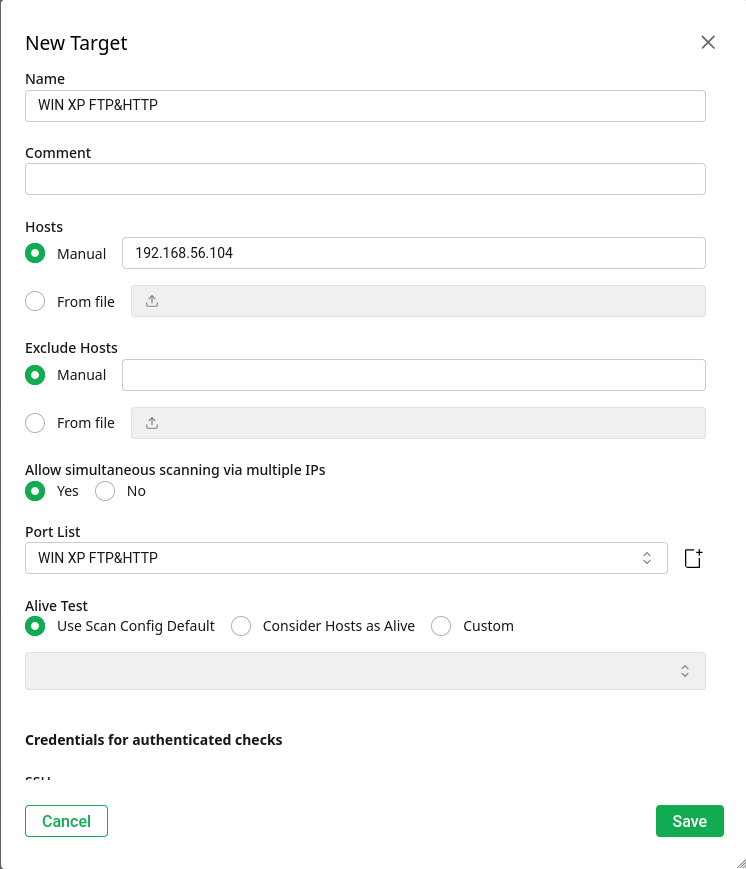
\includegraphics[width=\textwidth]{images/openvas_xpftphttp1.png}
        \caption{FTP \& HTTP Target Step 1} 
        \label{fig:ftphttptarget1}
    \end{subfigure}
    \hfill 
    \begin{subfigure}{0.48\textwidth}
        \centering
        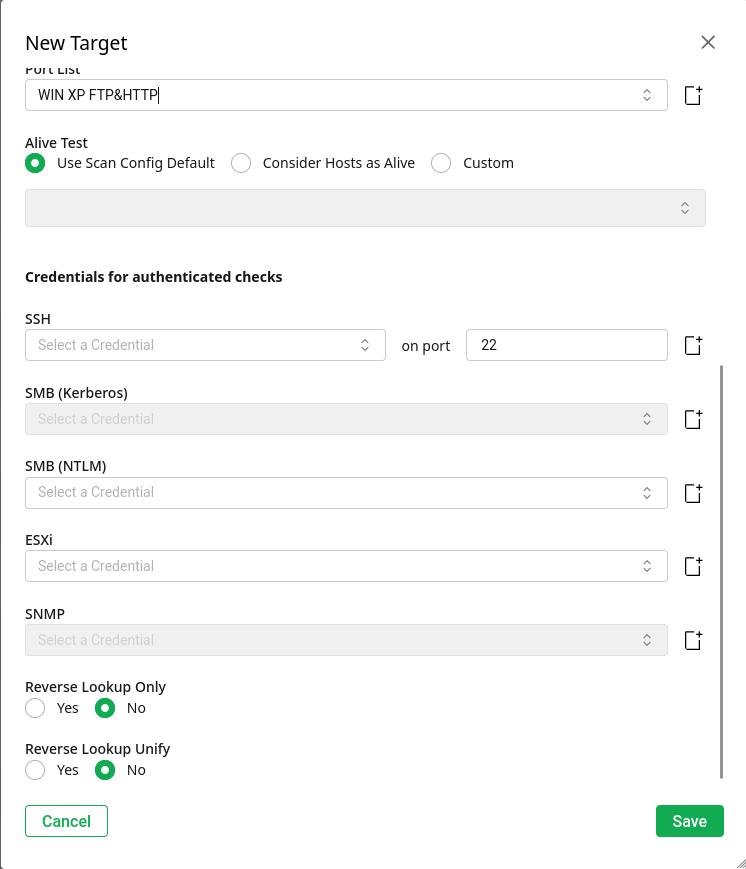
\includegraphics[width=\textwidth]{images/openvas_xpftphttp2.png}
        \caption{FTP \& HTTP Target Step 2}
        \label{fig:ftphttptarget2}
    \end{subfigure}
    \caption{Configuration for the FTP \& HTTP target}
    \label{fig:full_target_config_http}
\end{figure}


\subsubsection{Scan configs}


\begin{figure}[H]
    \centering
    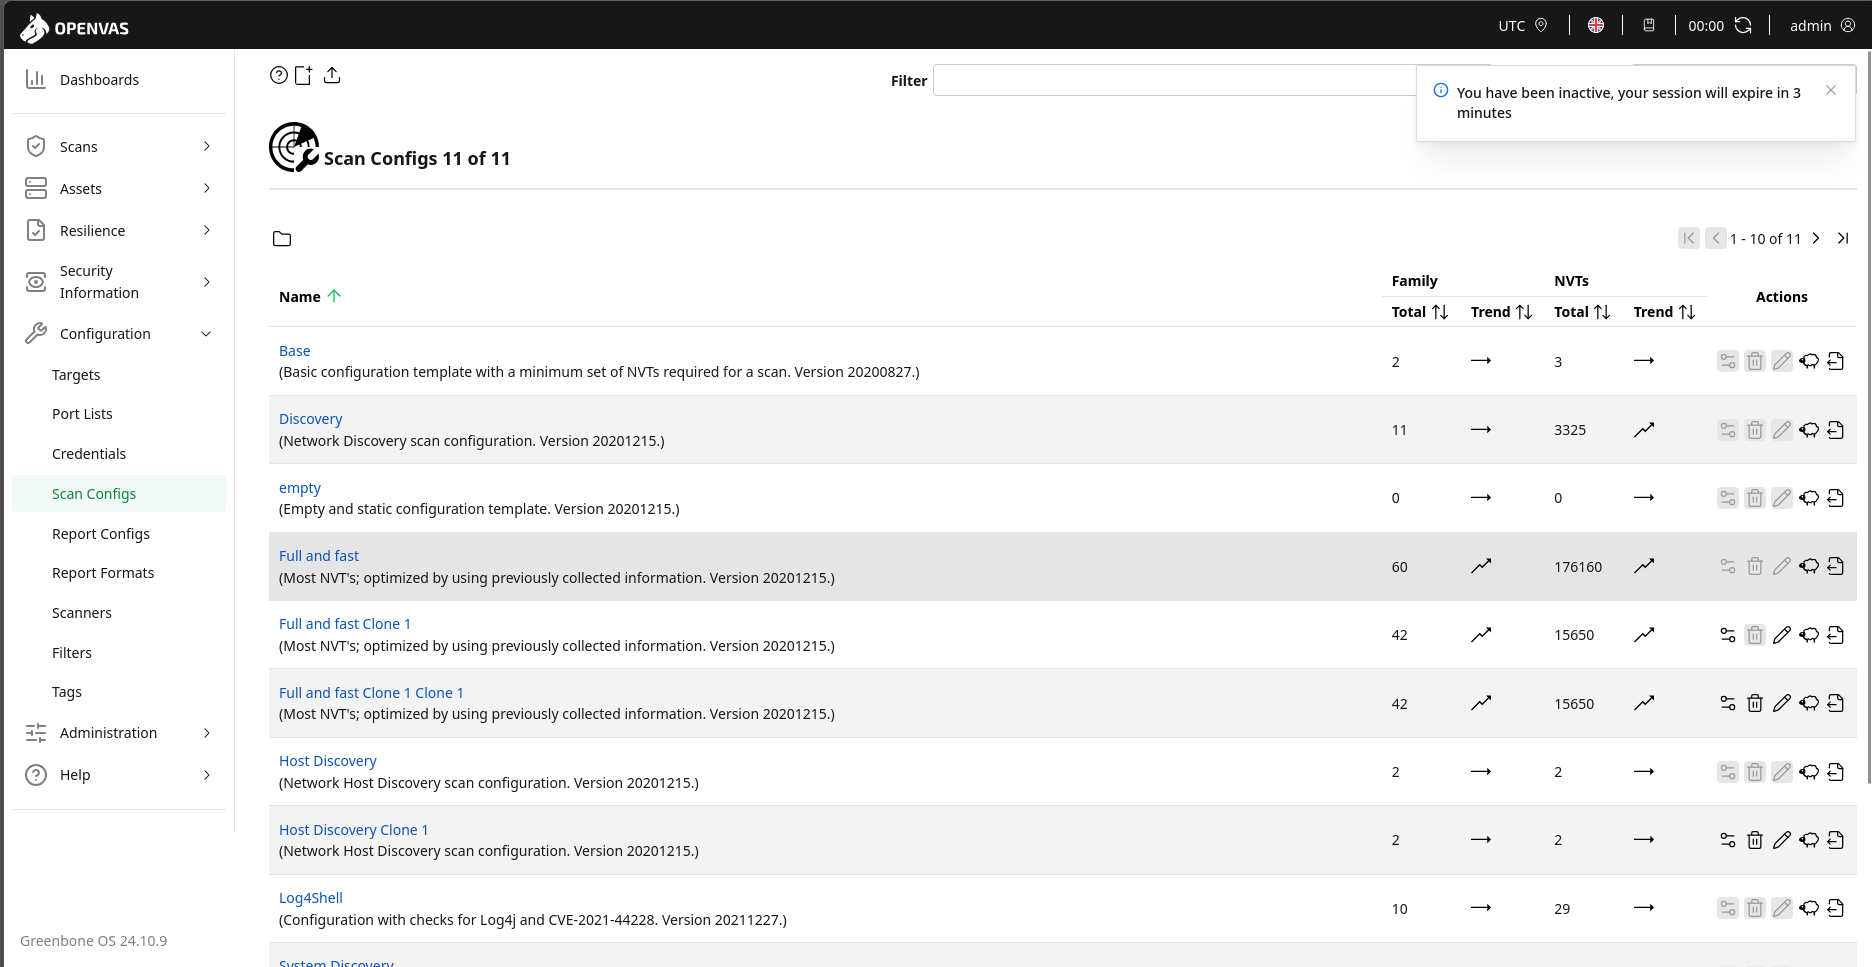
\includegraphics[width=0.8\textwidth]{images/openvas_scanconfigs.png}
    \caption{Scan configs window}
\end{figure}

The scan configuration is a configuration used during the scan, essentially it tells OpenVAS how to scan and what to scan. Essentially the Full and Fast preset looks at everything possible from Cisco appliances, Fedora security, Windows services etc. This is the reason why the database is so big, occupying tens of gigabytes. Since there are thousands of settings if we look at every possible configuration, what we will do is to configure a pre-set at a high level tayloring it for Windows XP.

\begin{figure}[H]
    \centering
    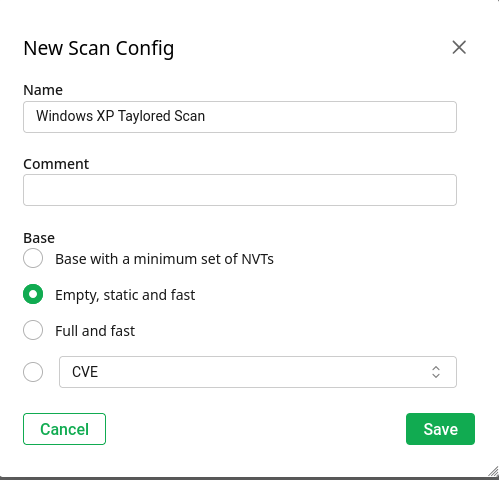
\includegraphics[width=0.8\textwidth]{images/openvas_tayloredscan.png}
    \caption{Taylored scan creation}
\end{figure}

To create it select the Empty config, save it and then edit it by clicking to the pencil icon, select the following:

\begin{figure}[H]
    \centering
    \begin{subfigure}{0.48\textwidth}
        \centering
        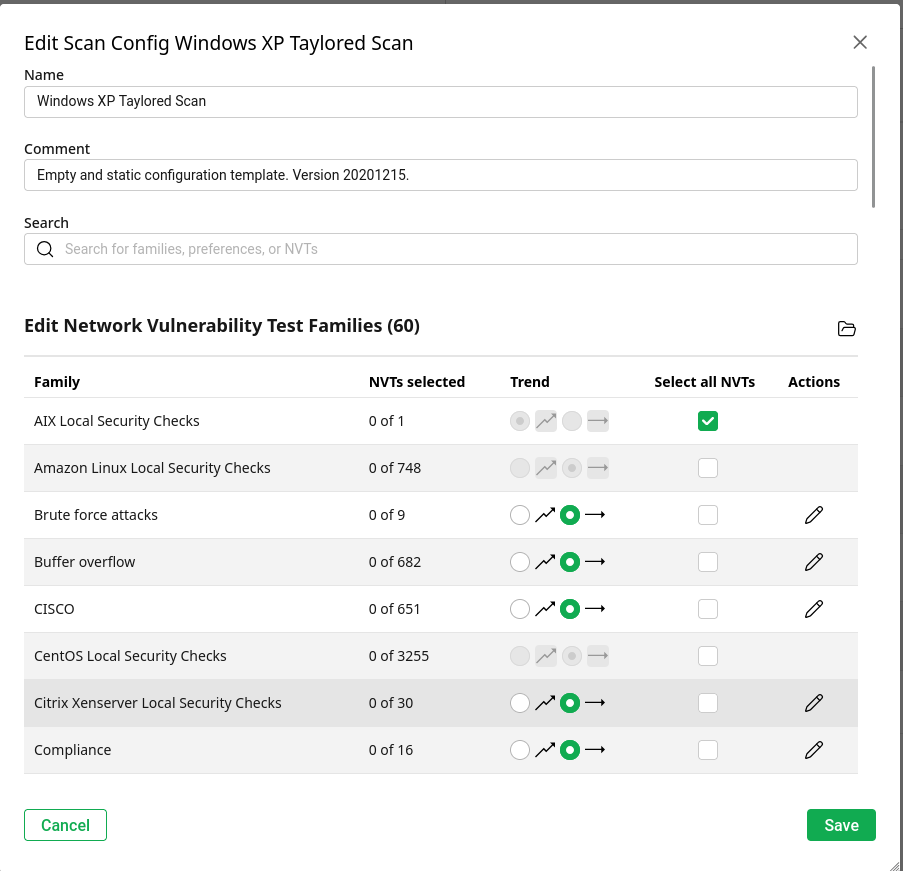
\includegraphics[width=\textwidth]{images/openvas_tayloredscan1.png}
        \caption{FTP \& HTTP Taylored scan options 1} 
        \label{fig:ftphttptaylored1}
    \end{subfigure}
    \hfill 
    \begin{subfigure}{0.48\textwidth}
        \centering
        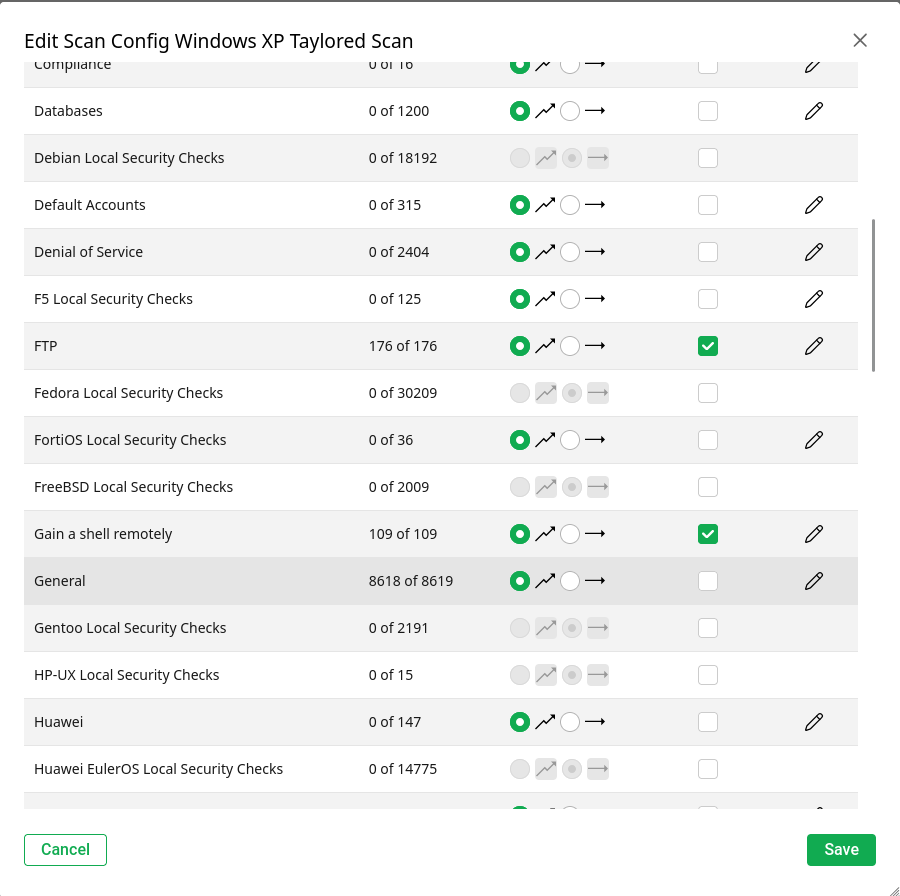
\includegraphics[width=\textwidth]{images/openvas_tayloredscan2.png}
        \caption{FTP \& HTTP Taylored scan options 2}
        \label{fig:ftphttptaylored2}
    \end{subfigure}
    \label{fig:ftphttptayloredscan1}
\end{figure}

\begin{figure}[H]
    \centering
    \begin{subfigure}{0.48\textwidth}
        \centering
        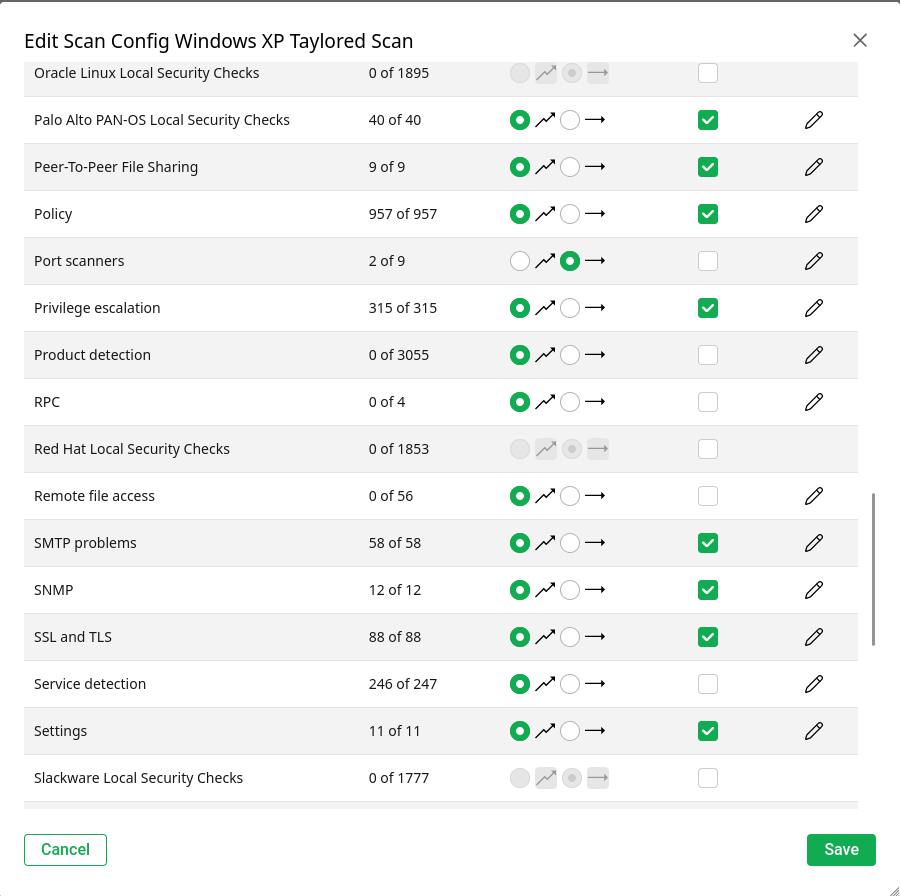
\includegraphics[width=\textwidth]{images/openvas_tayloredscan3.png}
        \caption{FTP \& HTTP Taylored scan options 3} 
        \label{fig:ftphttptaylored3}
    \end{subfigure}
    \hfill 
    \begin{subfigure}{0.48\textwidth}
        \centering
        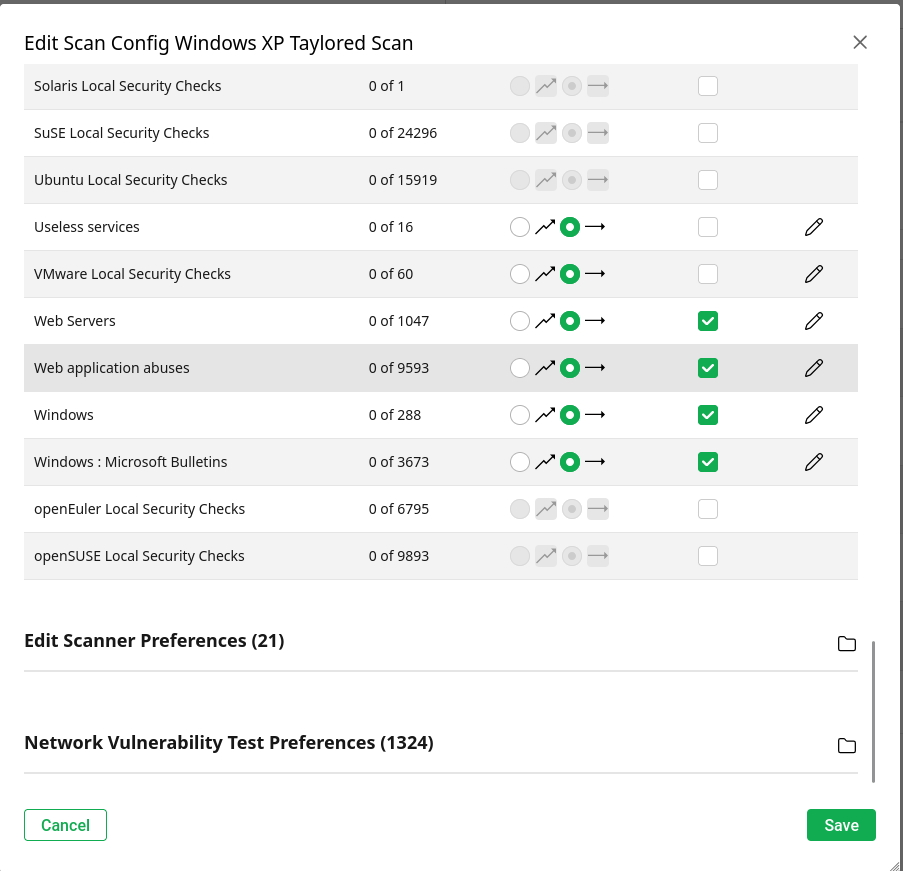
\includegraphics[width=\textwidth]{images/openvas_tayloredscan4.png}
        \caption{FTP \& HTTP Taylored scan options 4}
        \label{fig:ftphttptaylored4}
    \end{subfigure}
    \caption{Configuration for the FTP \& HTTP taylored scan}
    \label{fig:ftphttptayloredscan2}
\end{figure}

\subsection{Starting the scan}
Now we are ready to begin the scan, to do this go back to the tasks windows, click on the task add button and do the following:



\begin{figure}[H]
    \centering
    \begin{subfigure}{0.48\textwidth}
        \centering
        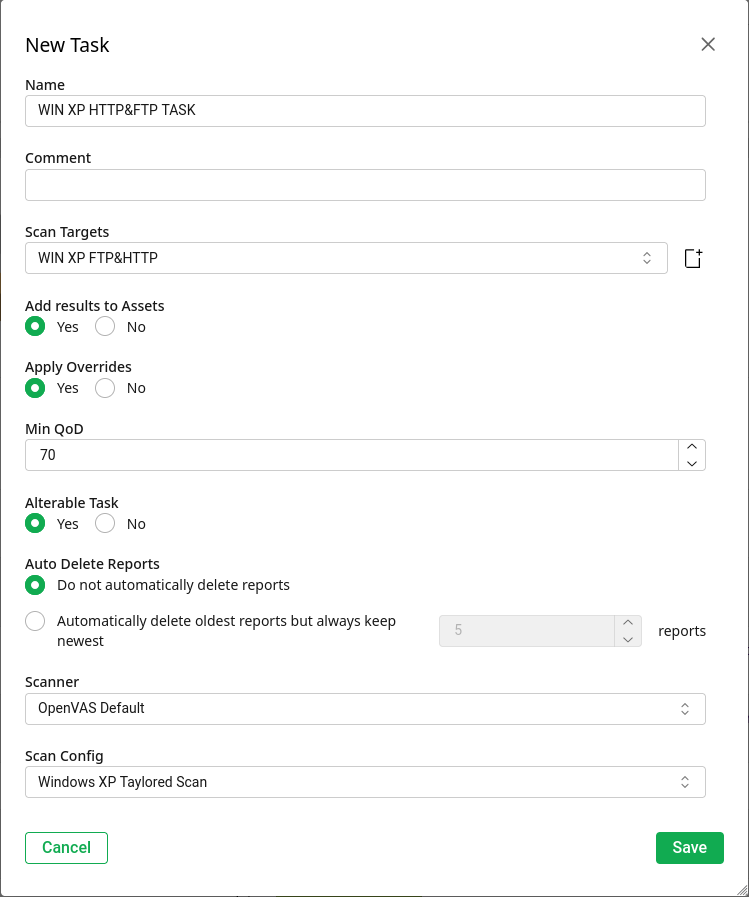
\includegraphics[width=\textwidth]{images/openvas_tayloredtask1.png}
        \caption{FTP \& HTTP Taylored task 1} 
        \label{fig:ftphttptayloredtask1}
    \end{subfigure}
    \hfill 
    \begin{subfigure}{0.48\textwidth}
        \centering
        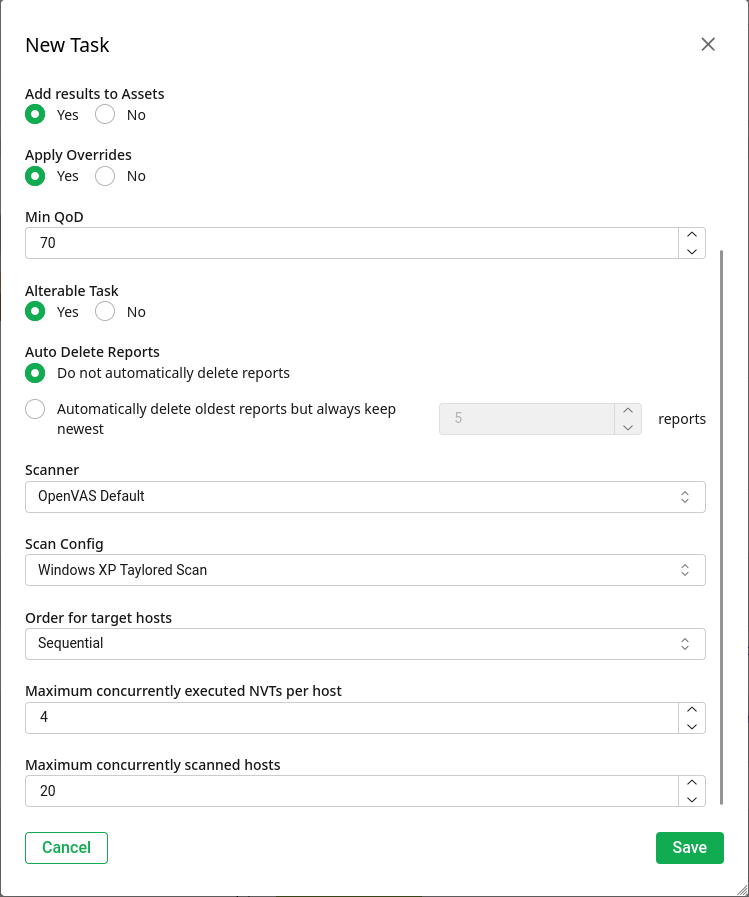
\includegraphics[width=\textwidth]{images/openvas_tayloredtask2.png}
        \caption{FTP \& HTTP Taylored task 2}
        \label{fig:ftphttptayloredtask2}
    \end{subfigure}
    \label{fig:ftphttptayloredtask1}
\end{figure}

